\section{Enclave Operation}

SGX provides trusted computing by protecting the privacy and integrity of the
computation that is performed inside an enclave, and by providing remote
attestation identifying the software running inside an enclavee. This section
describes the processes used to set up an enclave and perform computation
inside it.

% TODO: find a place for the rest of this section
% Access Control Requirements: SDM S 38.3

Enclave code runs at ring 3 (\S~\ref{sec:rings}), just like application code,
so that it cannot interfere with the system software that manages resources.

% Interactions with VMX: SDM S 42.5, S 42.5.{1,2,3,4,5}

On most computers, the system software that manages SGX resources is an
operating system kernel. When VMX is in use, the hypervisor is responsible for
multiplexing SGX resources across the guest operating systems running in
virtual machines.


\subsection{Evicting EPC Pages}
\label{sec:sgx_ewb}

% Eviction of Enclave Pages: SDM S 39.5.3
% Eviction of an SECS Page: SDM S 39.5.5
% Eviction of a Version Array Page: SDM S 39.5.6

% EPA: SDM S 41.3

\begin{figure}[hbt!]
  \centering
  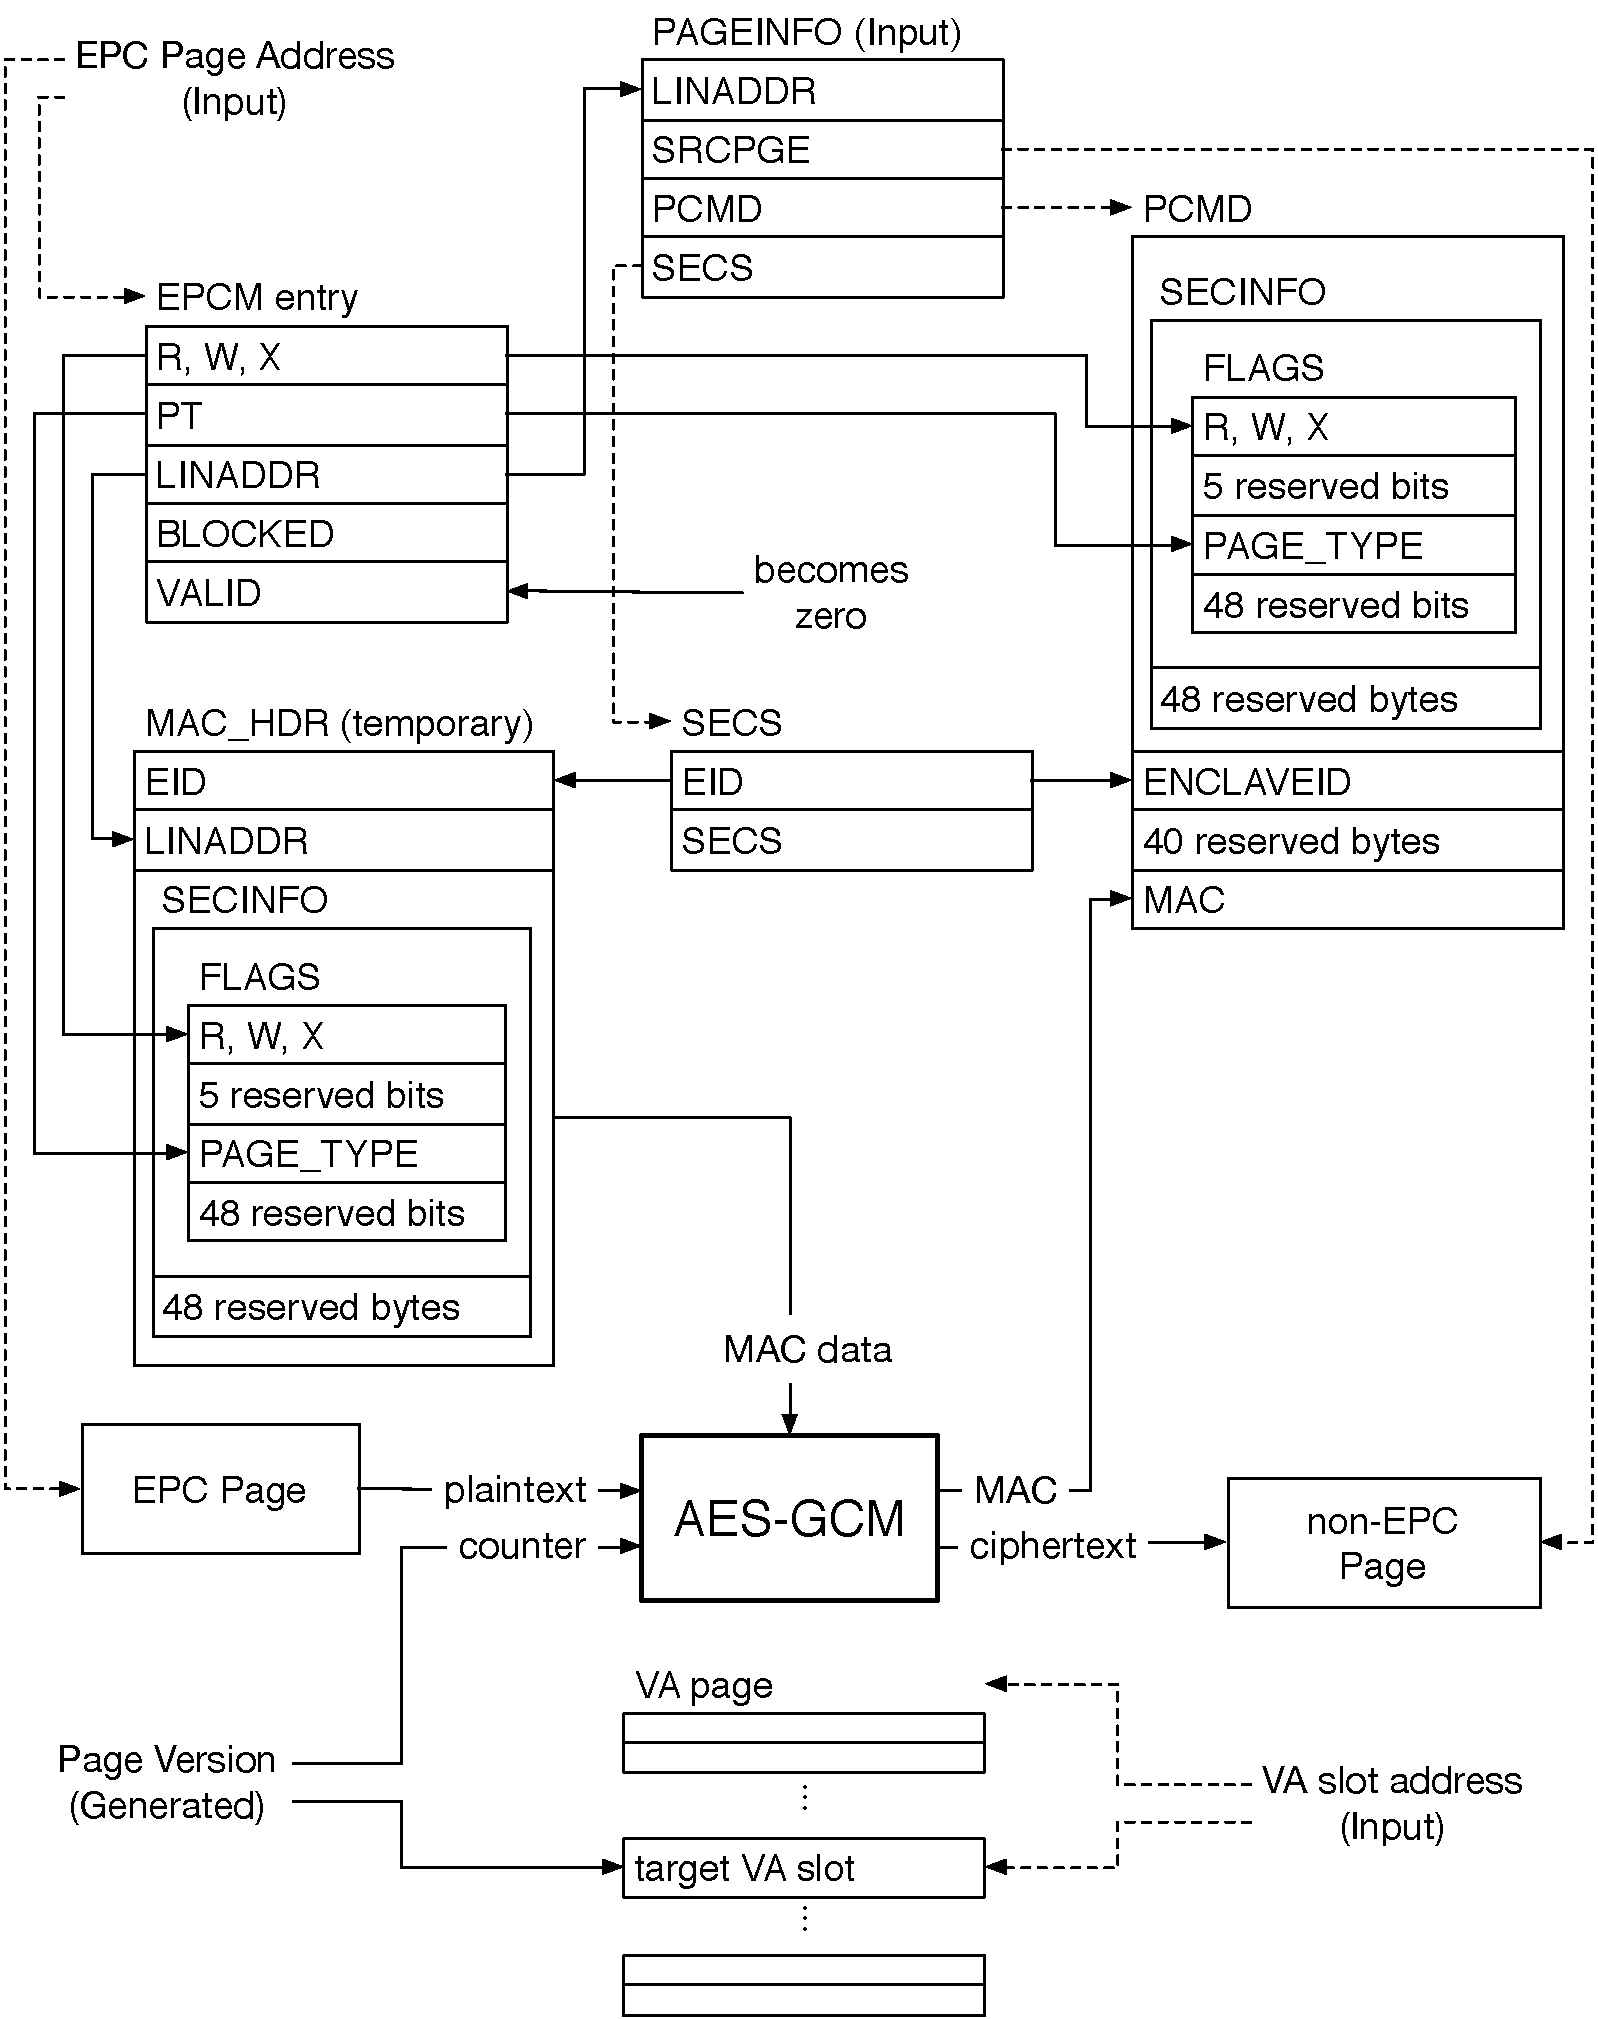
\includegraphics[width=85mm]{figures/sgx_ewb.pdf}
  \caption{
    The data flow of the EWB instruction that evicts an EPC page. The page's
    content is encrypted in a non-EPC RAM page. A nonce is created and saved
    in an empty slot inside a VA page. The page's EPCM metadata and a MAC
    are saved in a separate area in non-EPC memory.
  }
  \label{fig:sgx_ewb}
\end{figure}

% Loading an Enclave Page: SDM S 39.5.4


